

\actTitle{Worksheet 4.5B}

\noindent \textbf{Instructions:}  Work together in groups of  3 or 4 to complete the following problems.\\

\begin{enumerate}

\item Write an equation of the form $A\cos(Bx+C)+D$ for the given graph where $A>0$ and  $B>0$.
\begin{center}
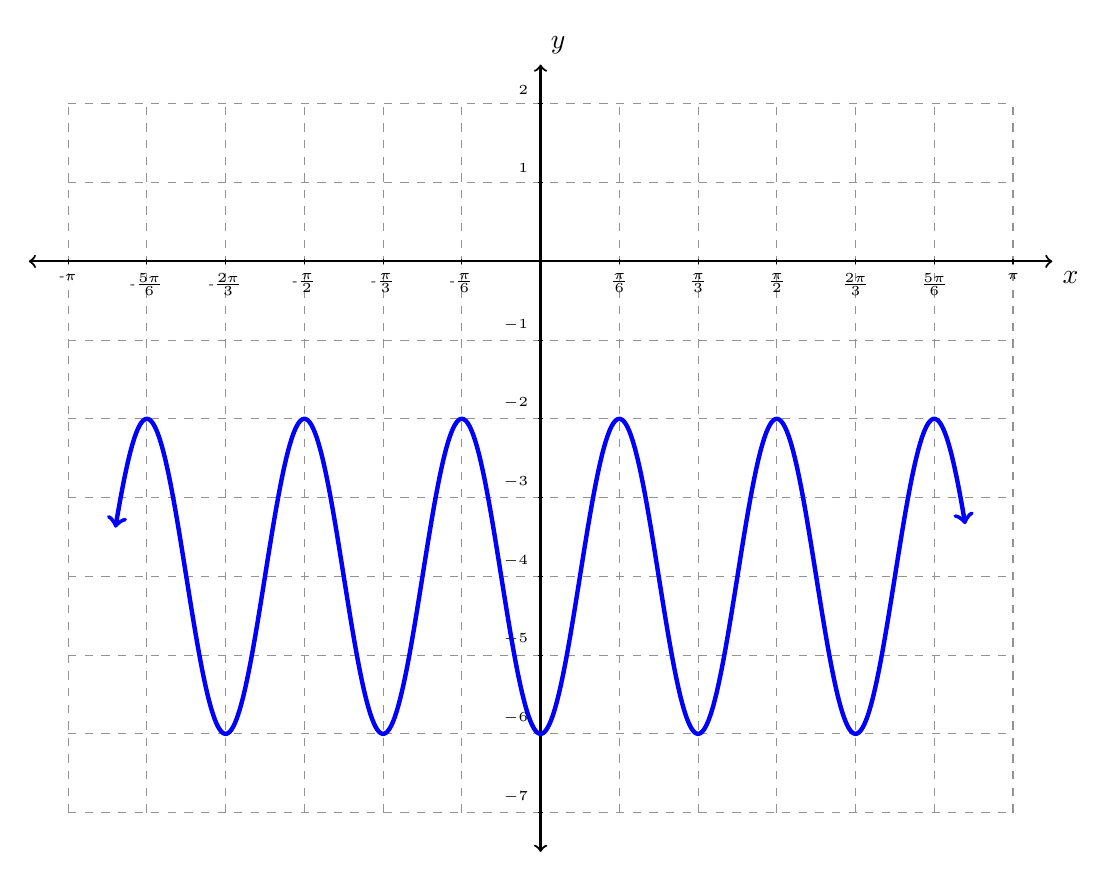
\begin{tikzpicture}[y=1cm, x=1cm,font=\sffamily,
	mydot/.style={
    circle,
    fill=white,
    draw,
    outer sep=0pt,
    inner sep=1.5pt
  }]
    %% Add a grid
    \draw[step = 1, gray, dashed,opacity=0.85] (-6, -7) grid (6, 2);
 	%% Draw the axes
	\draw[thick,<->] (-6.5,0) -- coordinate (x axis mid) (6.5,0) node[anchor = north west] {$x$};
    \draw[thick,<->] (0,-7.5) -- coordinate (y axis mid) (0,2.5) node[anchor = south west] {$y$};
    %% Label the y axis
    \foreach \y in {-7,...,-1,1,2,...,2} {
      \draw (1pt, \y) -- (-1pt, \y) node[anchor = south east] {\tiny $\y$};
    }
    %% Label the x axis
    %\foreach \x in {-5,...,-1,1,2,...,5} {
    %  \draw (\x,1pt) -- (\x,-1pt) node[anchor = north] {\tiny $\x$};
    %}
    \draw (-6,1pt) -- (-6,-1pt) node[anchor = north] {\tiny -$\pi$};
    \draw (-5,1pt) -- (-5,-1pt) node[anchor = north] {\tiny -$\frac{5\pi}{6}$};
    \draw (-4,1pt) -- (-4,-1pt) node[anchor = north] {\tiny -$\frac{2\pi}{3}$};
    \draw (-3,1pt) -- (-3,-1pt) node[anchor = north] {\tiny -$\frac{\pi}{2}$};
    \draw (-2,1pt) -- (-2,-1pt) node[anchor = north] {\tiny -$\frac{\pi}{3}$};
    \draw (-1,1pt) -- (-1,-1pt) node[anchor = north] {\tiny -$\frac{\pi}{6}$};
    \draw (1,1pt) -- (1,-1pt) node[anchor = north] {\tiny $\frac{\pi}{6}$};
    \draw (2,1pt) -- (2,-1pt) node[anchor = north] {\tiny $\frac{\pi}{3}$};
    \draw (3,1pt) -- (3,-1pt) node[anchor = north] {\tiny $\frac{\pi}{2}$};
    \draw (4,1pt) -- (4,-1pt) node[anchor = north] {\tiny $\frac{2\pi}{3}$};
    \draw (5,1pt) -- (5,-1pt) node[anchor = north] {\tiny $\frac{5\pi}{6}$};
    \draw (6,1pt) -- (6,-1pt) node[anchor = north] {\tiny $\pi$};

    %% Draw the function.
    \begin{scope}
%         \draw[very thick,blue] (-3,2) -- (1,1);
%         \draw[very thick,blue] (3.05,1.05) -- (4,3);
%         \draw[very thick,blue] (1.1,4) -- (3,4);
    %semi-circle
         %\draw[very thick, blue] (1,1) arc [radius=1, start angle=180, end angle= 5];
     %parabola
         %\draw[ultra thick, blue, domain=-5:0] plot (\x, {(-0.2)*(\x-5)*(\x+5)});
         \draw[ultra thick, blue, <->, domain=-5.4:5.4] plot[samples=1000] (\x, {-2*cos(pi*\x r)-4});             %dots
%         \fill[blue] (-3, 2) circle[radius=0.5ex];
%         \fill[blue] (1,1) circle[radius=0.5ex];
%         \fill[blue] (4,3) circle[radius=0.5ex];
%         \draw[very thick, blue] (3,1) circle[radius=0.5ex];
%         \fill[blue] (3,4) circle[radius=0.5ex];
%         \draw[very thick, blue] (1,4) circle[radius=0.5ex];


    \end{scope}

    %%\node[above=0.1cm] at (-2,2 )   {\nextXValue};

\end{tikzpicture}

\end{center}

\vfill


\clearpage
\item Write an equation of the form $A\sin(Bx+C)+D$ for the given graph where $A>0$ and  $B>0$.
\begin{center}
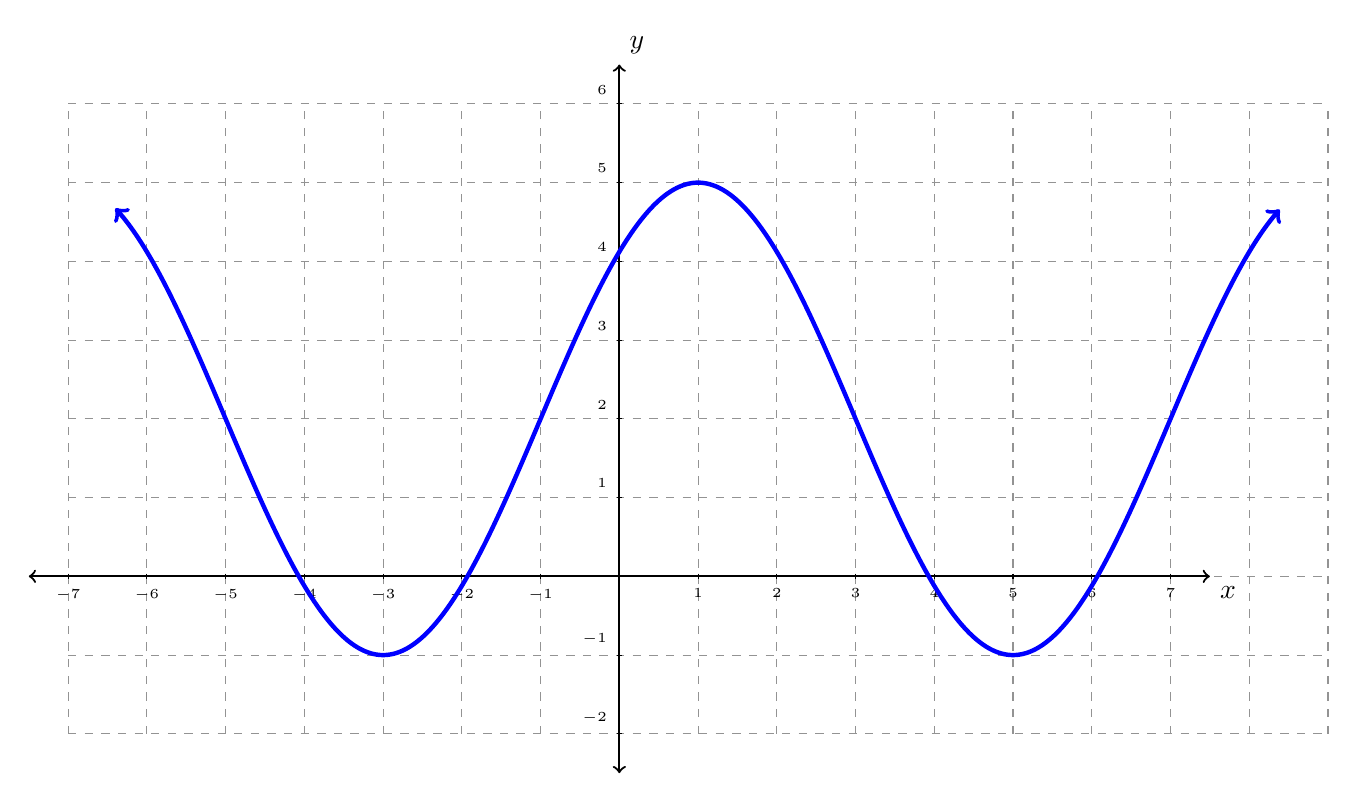
\begin{tikzpicture}[y=1cm, x=1cm,font=\sffamily,
	mydot/.style={
    circle,
    fill=white,
    draw,
    outer sep=0pt,
    inner sep=1.5pt
  }]
    %% Add a grid
    \draw[step = 1, gray,dashed,opacity=0.85] (-7, -2) grid (9, 6);
 	%% Draw the axes
	\draw[thick,<->] (-7.5,0) -- coordinate (x axis mid) (7.5,0) node[anchor = north west] {$x$};
    \draw[thick,<->] (0,-2.5) -- coordinate (y axis mid) (0,6.5) node[anchor = south west] {$y$};
    %% Label the y axis
    \foreach \y in {-2,...,-1,1,2,...,5,6} {
      \draw (1pt, \y) -- (-1pt, \y) node[anchor = south east] {\tiny $\y$};
    }
    %% Label the x axis
    \foreach \x in {-7,...,-1,1,2,...,7} {
      \draw (\x,1pt) -- (\x,-1pt) node[anchor = north] {\tiny $\x$};
    }
    %% Draw the function.
    \begin{scope}
%         \draw[very thick,blue] (-3,2) -- (1,1);
%         \draw[very thick,blue] (3.05,1.05) -- (4,3);
%         \draw[very thick,blue] (1.1,4) -- (3,4);
    %semi-circle
         %\draw[very thick, blue] (1,1) arc [radius=1, start angle=180, end angle= 5];
     %parabola
         %\draw[ultra thick, blue, domain=-5:0] plot (\x, {(-0.2)*(\x-5)*(\x+5)});
         \draw[ultra thick, blue, <->, domain=-6.4:8.4] plot[samples=1000] (\x, {3*sin(pi/4*(\x+1) r)+2});             %dots
%         \fill[blue] (-3, 2) circle[radius=0.5ex];
%         \fill[blue] (1,1) circle[radius=0.5ex];
%         \fill[blue] (4,3) circle[radius=0.5ex];
%         \draw[very thick, blue] (3,1) circle[radius=0.5ex];
%         \fill[blue] (3,4) circle[radius=0.5ex];
%         \draw[very thick, blue] (1,4) circle[radius=0.5ex];


    \end{scope}

    %%\node[above=0.1cm] at (-2,2 )   {\nextXValue};

\end{tikzpicture}

\end{center}


\vfill

\clearpage
\item Write equations of the form $A\sin(Bx+C)+D$ \textbf{AND} $A\cos(Bx+C)+D$ and for the given graph where $A>0$ and  $B>0$.
\begin{center}
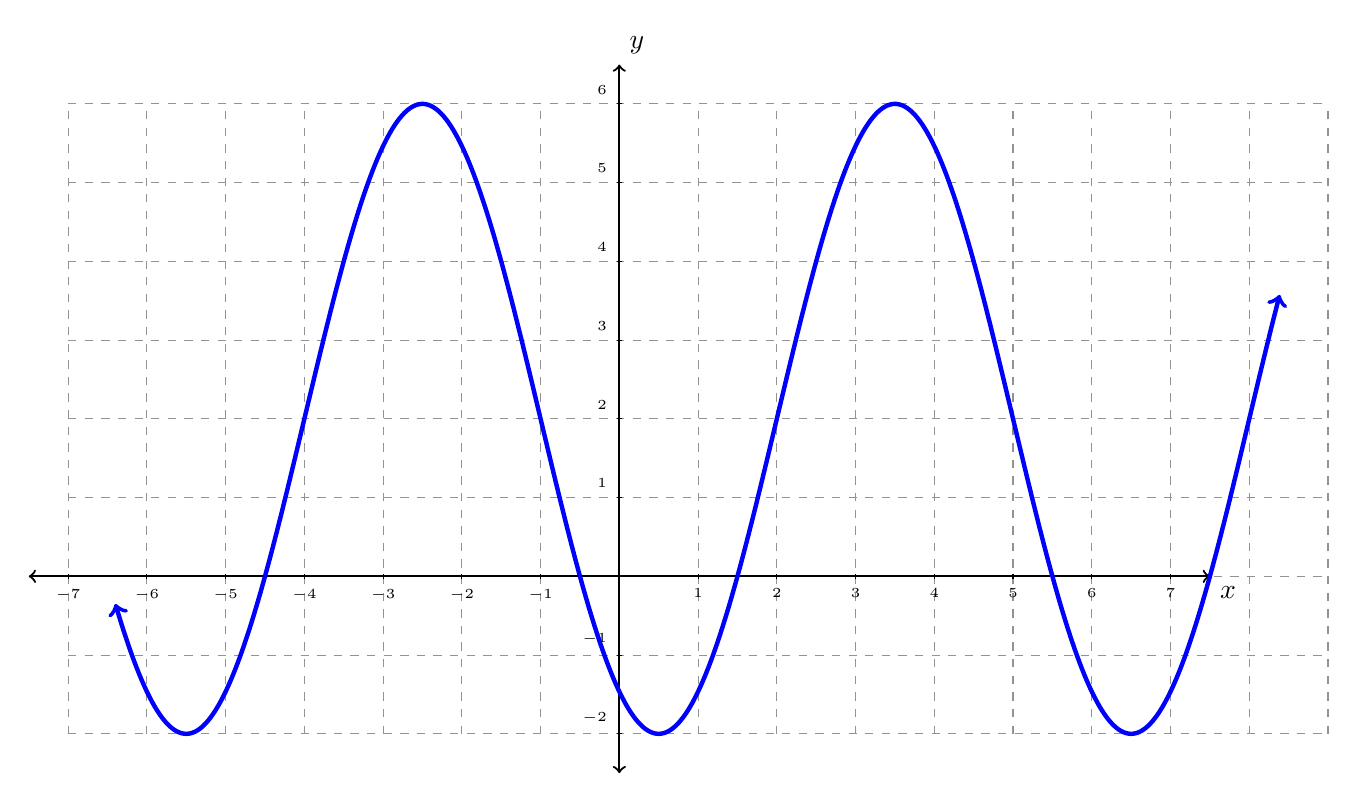
\begin{tikzpicture}[y=1cm, x=1cm,font=\sffamily,
	mydot/.style={
    circle,
    fill=white,
    draw,
    outer sep=0pt,
    inner sep=1.5pt
  }]
    %% Add a grid
    \draw[step = 1, gray,dashed,opacity=0.85] (-7, -2) grid (9, 6);
 	%% Draw the axes
	\draw[thick,<->] (-7.5,0) -- coordinate (x axis mid) (7.5,0) node[anchor = north west] {$x$};
    \draw[thick,<->] (0,-2.5) -- coordinate (y axis mid) (0,6.5) node[anchor = south west] {$y$};
    %% Label the y axis
    \foreach \y in {-2,...,-1,1,2,...,5,6} {
      \draw (1pt, \y) -- (-1pt, \y) node[anchor = south east] {\tiny $\y$};
    }
    %% Label the x axis
    \foreach \x in {-7,...,-1,1,2,...,7} {
      \draw (\x,1pt) -- (\x,-1pt) node[anchor = north] {\tiny $\x$};
    }
    %% Draw the function.
    \begin{scope}
%         \draw[very thick,blue] (-3,2) -- (1,1);
%         \draw[very thick,blue] (3.05,1.05) -- (4,3);
%         \draw[very thick,blue] (1.1,4) -- (3,4);
    %semi-circle
         %\draw[very thick, blue] (1,1) arc [radius=1, start angle=180, end angle= 5];
     %parabola
         %\draw[ultra thick, blue, domain=-5:0] plot (\x, {(-0.2)*(\x-5)*(\x+5)});
          \draw[ultra thick, blue, <->, domain=-6.4:8.4] plot[samples=1000] (\x, {-4*sin(pi/3*(\x+1) r)+2});             %dots
%         \fill[blue] (-3, 2) circle[radius=0.5ex];
%         \fill[blue] (1,1) circle[radius=0.5ex];
%         \fill[blue] (4,3) circle[radius=0.5ex];
%         \draw[very thick, blue] (3,1) circle[radius=0.5ex];
%         \fill[blue] (3,4) circle[radius=0.5ex];
%         \draw[very thick, blue] (1,4) circle[radius=0.5ex];


    \end{scope}

    %%\node[above=0.1cm] at (-2,2 )   {\nextXValue};

\end{tikzpicture}

\end{center}


\vfill




\clearpage
\item The water level relative to the top of a boat dock varies with
  the tides.  One particular day, low tide occurs at midnight and the
  water level is 7ft below the dock.  The first high tide of the day
  occurs at approximately 6:00 AM, and the water level is 3ft below
  the dock.  The next low tide occurs at noon and the water level is
  again 7ft below the dock.
  
  Assuming that this pattern continues indefinitely and behaves like a
  cosine wave, write a function of the form $w(t)=A\cos(Bt+C)+D$.  The
  value $w(t)$ is the water level (in ft) relative to the top of the
  dock, $t$ hours after midnight.

  \vfill

\clearpage

\item The function $f(x)=A\sin(Bx)+D$ has a period of $13\pi$.  If the graph of $f(x)$ oscillates between 2 and 20, determine the numeric values for A, B, and D.  (You may assume that A, B, and D are positive.)
\vfill
\vfill

\item Write the range of the function in interval notation.
\begin{enumerate}
\item $y=\sin(x)$\\[0.2in]
\item $y=\cos(x)$\\[0.2in]
\item $y=8\cos(2x-\pi)+4$\vfill
\end{enumerate}

\clearpage


\item The London Eye is a Ferris wheel with a diameter of 120
  meters. The center of the wheel is 75 meters above the ground, and
  the wheel makes one revolution every thirty minutes. If one of the
  capsules is initially at the lowest level at the initial time,
  determine a function that returns the height of the capsule above
  the ground given the number of minutes after the initial time.

  \vfill


\end{enumerate}


\hwTitle{Section 4.5B}

\begin{enumerate}
\item Write the range of the function in interval notation.
\begin{enumerate}
\item $y=-3\cos\left(x+\frac{\pi}{3}\right)-5$
\item $y=-6\sin\left(3x-\frac{\pi}{2}\right)-2$
\item $y=-\sin(x)$
\item $y=-5\cos(2x+1)+ 10$
\item $y=20\cos\left(5x-\frac{\pi}{5}\right)+20$
\end{enumerate}

\item Graph $f(x)=-6\sin\left(3x-\frac{\pi}{2}\right)-2$.

\begin{tikzpicture}[y=.6cm, x=1.3cm,font=\sffamily]
    %% ticks
    \draw[step = 1, gray,dashed] (-5,-10) grid (5,10);
    %% axis
    \draw[thick,->] (-5.5,0) -- coordinate (x axis mid) (5.5,0) node[anchor = north west] {$x$};
    \draw[thick,->] (0,-10.5) -- coordinate (y axis mid) (0,10.5) node[anchor = north east] {$y$};
    %\foreach \y in {-10,-9,...,-1,1,2,...,10} {
    %  \draw (2pt, \y) -- (-2pt, \y);
    %}
    %\foreach \x in {-6,-5,...,-1,1,2,...,6} {
    %  \draw (\x,2pt) -- (\x,-2pt);
    %}

  \end{tikzpicture}

\item Determine a formula for the sine wave that oscillates between
  two and eight. It has a minimum at $x = 2$, and the wave repeats
  every five units (i.e. the period is five).

\item Determine a formula for the cosine wave that oscillates between
  minus five and twenty. It has a maximum at $x=6$, and the wave repeats
  every four units (i.e. the period is four).

\item The water level at a beach oscillates between 0.4m
  \textbf{below} the mean tidal level and 3.4m \textbf{above} the mean
  tidal level. The time between low and high tides is 6.4 hours. If
  low tide occurs at midnight, express the water level as a cosine
  function where the time is the number of hours past midnight,
  \begin{eqnarray*}
    h(t) & = & A \cos(bt+c)+d.
  \end{eqnarray*}

\item The water level at Jeffries Creek varies between 2.4 meters and
  0.2 meters due to the changes in the tide. The time between high
  tides is 700 minutes. The next high tide will occur at 150 minutes
  after midnight. Express the water level as a sine function assuming
  that $t=0$ minutes is midnight.

\item Determine the cosine function whose graph is shown below.

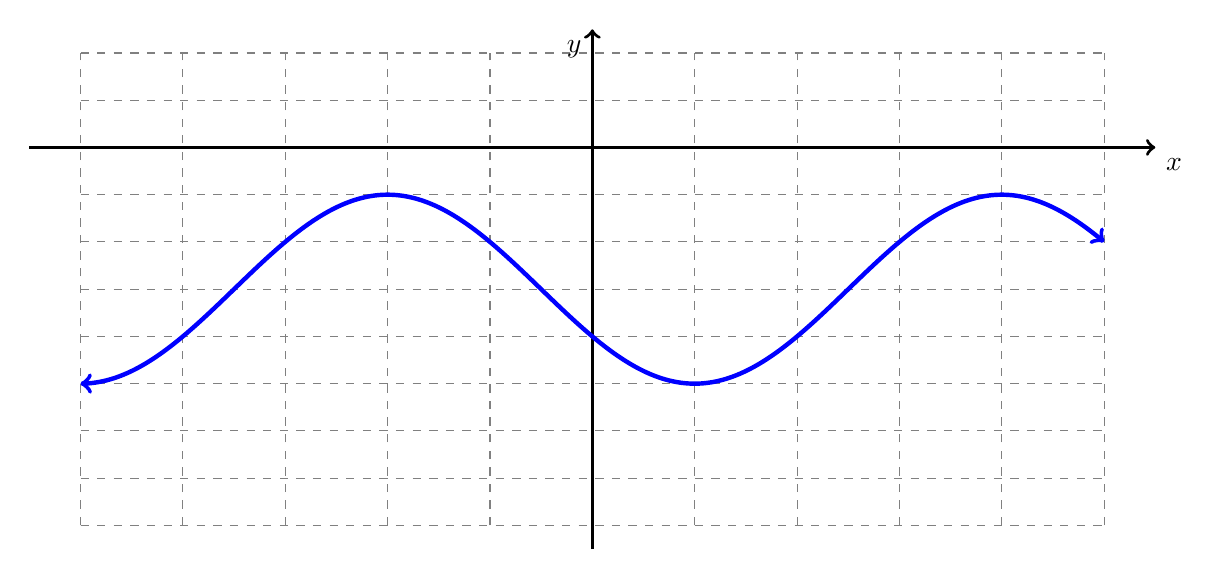
\begin{tikzpicture}[y=.6cm, x=1.3cm,font=\sffamily]
  %% ticks
  \draw[step = 1, gray,dashed] (-5,-8) grid (5,2);
  %% axis
  \draw[very thick,->] (-5.5,0) -- coordinate (x axis mid) (5.5,0) node[anchor = north west] {$x$};
  \draw[very thick,->] (0,-8.5) -- coordinate (y axis mid) (0,2.5) node[anchor = north east] {$y$};
  \draw[ultra thick, blue, <->, domain=-5:5] plot[samples=1000] (\x, {2*cos(deg(pi/3*(\x+2)))-3});
\end{tikzpicture}

\item The wheel used in the game show Wheel Of Fortune is
  approximately 2.6 meters in diameter. Suppose the Wheel is mounted
  vertically on a wall for a special event so that its center is 4
  meters above the floor. Initially, the 100\$ marker is to the right,
  and the Wheel is spun clock-wise so that it takes four seconds to
  make one revolution. Determine the height above the floor of the
  outside edge of the 100\$ marker given the number of seconds after
  the initial time.

\item The clock face of the Rajabai Tower is approximately 65 meters
  above the ground, and the length of the minute hand is approximately
  7.3 meters. A bird lands on the end of the minute hand at 3:45PM and
  remains on the minute for thirty minutes. Determine the bird's
  height above the ground given the number of minutes after 3:45PM.

\item The height above the ground (in meters) for the seats on a Ferris wheel is
  given by
  \begin{eqnarray*}
    H(t) & = & 27 \cos\left(\frac{\pi}{3}t+\pi\right) + 32,
  \end{eqnarray*}
  where $t$ is the time in minutes from the start of the
  ride. Determine how long it takes for one revolution to occur. How
  tall is the loading platform which is located at the bottom of the
  wheel? What is the maximum height of one of the seats?


\end{enumerate}
